\documentclass[tikz,border=2pt]{standalone}
\usepackage{xcolor}
\usetikzlibrary{arrows.meta,positioning}

\definecolor{ink}{HTML}{26363E}
\definecolor{muted}{HTML}{667781}
\definecolor{teal}{HTML}{167F78}
\definecolor{tealbg}{HTML}{EDF7F5}
\definecolor{blue}{HTML}{3973B7}
\definecolor{bluebg}{HTML}{EEF4FA}
\definecolor{violet}{HTML}{7657B5}
\definecolor{violetbg}{HTML}{F3F0FA}

\begin{document}
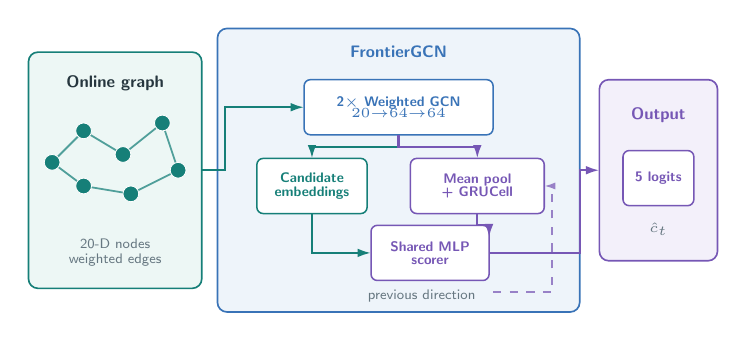
\begin{tikzpicture}[
  x=1mm,y=1mm,font=\sffamily,
  box/.style={rounded corners=1.2mm,line width=.6pt,align=center,inner sep=1.5mm},
  title/.style={font=\sffamily\bfseries\fontsize{6.3}{7.1}\selectfont,
                text=ink,align=center},
  sub/.style={font=\sffamily\fontsize{4.8}{5.5}\selectfont,
              text=muted,align=center},
  layer/.style={rounded corners=.8mm,line width=.55pt,align=center,
                minimum height=7mm,inner sep=.8mm,
                font=\sffamily\bfseries\fontsize{4.2}{4.8}\selectfont},
  tiny/.style={font=\sffamily\fontsize{3.5}{4.0}\selectfont,text=muted,align=center},
  flow/.style={-{Latex[length=1.7mm,width=1.1mm]},line width=.8pt},
  dot/.style={circle,fill=teal,draw=white,line width=.3pt,inner sep=0pt,
              minimum size=2mm}
]

% Online graph input.
\node[box,draw=teal,fill=tealbg,minimum width=22mm,minimum height=30mm]
  (input) at (13,23) {};
\node[title] at (13,34) {Online graph};
\node[sub] at (13,12.5) {20-D nodes\\weighted edges};

\draw[teal!75,line width=.65pt]
  (5,24)--(9,28)--(14,25)--(19,29)--(21,23)--(15,20)--(9,21)--(5,24);
\foreach \x/\y in {5/24,9/28,14/25,19/29,21/23,15/20,9/21} {
  \node[dot] at (\x,\y) {};
}

% Deployed graph policy. The encoded graph splits into candidate and temporal paths.
\node[box,draw=blue,fill=bluebg,minimum width=46mm,minimum height=36mm]
  (policy) at (49,23) {};
\node[title,text=blue] at (49,38) {FrontierGCN};

\node[layer,draw=blue,fill=white,text=blue,minimum width=24mm]
  (encoder) at (49,31) {2$\times$ Weighted GCN\\[-1pt]{\normalfont\tiny 20$\rightarrow$64$\rightarrow$64}};

\node[layer,draw=teal,fill=white,text=teal,minimum width=14mm]
  (cand) at (38,21) {Candidate\\embeddings};
\node[layer,draw=violet,fill=white,text=violet,minimum width=17mm]
  (temporal) at (59,21) {Mean pool\\+ GRUCell};
\node[layer,draw=violet,fill=white,text=violet,minimum width=15mm]
  (mlp) at (53,12.5) {Shared MLP\\scorer};

\draw[flow,draw=teal] (49,27.5)--(49,26)--(38,26)--(38,24.5);
\draw[flow,draw=violet] (49,27.5)--(49,26)--(59,26)--(59,24.5);
\draw[flow,draw=teal] (38,17.5)--(38,12.5)--(45.5,12.5);
\draw[flow,draw=violet] (59,17.5)--(59,16)--(60.5,16)--(60.5,14.5);

\node[tiny,anchor=east] at (60,7) {previous direction};
\draw[-{Latex[length=1.4mm,width=.9mm]},violet!75,dashed,line width=.65pt]
  (61,7.5)--(68.5,7.5)--(68.5,21)--(67.5,21);

% Small output stage; geometric validation remains outside the network.
\node[box,draw=violet,fill=violetbg,minimum width=15mm,minimum height=23mm]
  (output) at (82,23) {};
\node[title,text=violet] at (82,30) {Output};
\node[layer,draw=violet,fill=white,text=violet,minimum width=9mm]
  at (82,22) {5 logits};
\node[sub] at (82,15.5) {$\hat c_t$};

\draw[flow,draw=teal] (24,23)--(27,23)--(27,31)--(37,31);
\draw[flow,draw=violet] (60.5,12.5)--(72,12.5)--(72,23)--(74.5,23);

\end{tikzpicture}
\end{document}
